% نوسانگر هماهنگ: پتانسیل و ترازها (طرحواره)
% سبک مشترک نمودارهای سند پایه‌ها (فقط داخل محیط latin فراخوانی شود)
\tikzset{
	qafbox/.style={
		draw=black!55,
		rounded corners=2pt,
		align=center,
		inner sep=3pt,
		thick,
		fill=white,
		font=\footnotesize\linespread{1}\selectfont,
		minimum height=0.95cm
	},
	qafwide/.style={
		qafbox,
		text width=2.55cm
	},
	qafnarr/.style={
		qafbox,
		text width=2.05cm
	},
	qaftitle/.style={
		font=\small\bfseries\linespread{1}\selectfont,
		align=center
	},
	qafarr/.style={
		-{Latex[length=2.2mm]},
		thick,
		draw=black!65
	},
	qafpanel/.style={
		draw,
		thick,
		rounded corners=4pt,
		inner xsep=8pt,
		inner ysep=8pt
	}
}

\begin{tikzpicture}[
	x=1.1cm,
	y=0.9cm,
	note/.style={font=\scriptsize, text=black!55}
	]
	\draw[->, thick] (-2.2,0) -- (2.4,0) node[right] {$x$};
	\draw[->, thick] (0,-0.3) -- (0,3.2) node[above] {$V(x)$};
	\draw[thick, blue!70!black, domain=-1.9:1.9, samples=60]
		plot (\x, {0.55*\x*\x});
	\draw[thick, black!50] (-1.55,1.3) -- (1.55,1.3);
	\draw[thick, black!50] (-1.85,1.95) -- (1.85,1.95);
	\draw[thick, black!50] (-2.05,2.55) -- (2.05,2.55);
	\node[note, right] at (1.6,1.3) {$E_0$};
	\node[note, right] at (1.9,1.95) {$E_1$};
	\node[note, right] at (2.1,2.55) {$E_2$};
	\node[note] at (0,-0.7) {$V=\tfrac12 m\omega^2 x^2$};
\end{tikzpicture}
